%%%%%%%%%%%%%%%%%%%%%%%%%%%%%%%%%%%%%%%%%
% University Assignment Title Page 
% LaTeX Template
% Version 1.0 (27/12/12)
%
% This template has been downloaded from:
% http://www.LaTeXTemplates.com
%
% Original author:
% WikiBooks (http://en.wikibooks.org/wiki/LaTeX/Title_Creation)
%
% License:
% CC BY-NC-SA 3.0 (http://creativecommons.org/licenses/by-nc-sa/3.0/)
% 
% Instructions for using this template:
% This title page is capable of being compiled as is. This is not useful for 
% including it in another document. To do this, you have two options: 
%
% 1) Copy/paste everything between \begin{document} and \end{document} 
% starting at \begin{titlepage} and paste this into another LaTeX file where you 
% want your title page.
% OR
% 2) Remove everything outside the \begin{titlepage} and \end{titlepage} and 
% move this file to the same directory as the LaTeX file you wish to add it to. 
% Then add %%%%%%%%%%%%%%%%%%%%%%%%%%%%%%%%%%%%%%%%%
% University Assignment Title Page 
% LaTeX Template
% Version 1.0 (27/12/12)
%
% This template has been downloaded from:
% http://www.LaTeXTemplates.com
%
% Original author:
% WikiBooks (http://en.wikibooks.org/wiki/LaTeX/Title_Creation)
%
% License:
% CC BY-NC-SA 3.0 (http://creativecommons.org/licenses/by-nc-sa/3.0/)
% 
% Instructions for using this template:
% This title page is capable of being compiled as is. This is not useful for 
% including it in another document. To do this, you have two options: 
%
% 1) Copy/paste everything between \begin{document} and \end{document} 
% starting at \begin{titlepage} and paste this into another LaTeX file where you 
% want your title page.
% OR
% 2) Remove everything outside the \begin{titlepage} and \end{titlepage} and 
% move this file to the same directory as the LaTeX file you wish to add it to. 
% Then add %%%%%%%%%%%%%%%%%%%%%%%%%%%%%%%%%%%%%%%%%
% University Assignment Title Page 
% LaTeX Template
% Version 1.0 (27/12/12)
%
% This template has been downloaded from:
% http://www.LaTeXTemplates.com
%
% Original author:
% WikiBooks (http://en.wikibooks.org/wiki/LaTeX/Title_Creation)
%
% License:
% CC BY-NC-SA 3.0 (http://creativecommons.org/licenses/by-nc-sa/3.0/)
% 
% Instructions for using this template:
% This title page is capable of being compiled as is. This is not useful for 
% including it in another document. To do this, you have two options: 
%
% 1) Copy/paste everything between \begin{document} and \end{document} 
% starting at \begin{titlepage} and paste this into another LaTeX file where you 
% want your title page.
% OR
% 2) Remove everything outside the \begin{titlepage} and \end{titlepage} and 
% move this file to the same directory as the LaTeX file you wish to add it to. 
% Then add %%%%%%%%%%%%%%%%%%%%%%%%%%%%%%%%%%%%%%%%%
% University Assignment Title Page 
% LaTeX Template
% Version 1.0 (27/12/12)
%
% This template has been downloaded from:
% http://www.LaTeXTemplates.com
%
% Original author:
% WikiBooks (http://en.wikibooks.org/wiki/LaTeX/Title_Creation)
%
% License:
% CC BY-NC-SA 3.0 (http://creativecommons.org/licenses/by-nc-sa/3.0/)
% 
% Instructions for using this template:
% This title page is capable of being compiled as is. This is not useful for 
% including it in another document. To do this, you have two options: 
%
% 1) Copy/paste everything between \begin{document} and \end{document} 
% starting at \begin{titlepage} and paste this into another LaTeX file where you 
% want your title page.
% OR
% 2) Remove everything outside the \begin{titlepage} and \end{titlepage} and 
% move this file to the same directory as the LaTeX file you wish to add it to. 
% Then add \input{./title_page_1.tex} to your LaTeX file where you want your
% title page.
%
%%%%%%%%%%%%%%%%%%%%%%%%%%%%%%%%%%%%%%%%%
%\title{Title page with logo}
%----------------------------------------------------------------------------------------
%	PACKAGES AND OTHER DOCUMENT CONFIGURATIONS
%----------------------------------------------------------------------------------------

\documentclass[12pt]{article}
\usepackage[english]{babel}
\usepackage[utf8x]{inputenc}
\usepackage{amsmath}
\usepackage{graphicx}
\usepackage[colorinlistoftodos]{todonotes}

\begin{document}

\begin{titlepage}

\newcommand{\HRule}{\rule{\linewidth}{0.5mm}} % Defines a new command for the horizontal lines, change thickness here

\center % Center everything on the page
 
%----------------------------------------------------------------------------------------
%	HEADING SECTIONS
%----------------------------------------------------------------------------------------

\textsc{\LARGE Politenico di Milano}\\[1.5cm] % Name of your university/college
\textsc{\Large Dipartimento Elettronica, Informazione e Bioingegneria}\\[0.5cm] % Major heading such as course name
\textsc{\large HEAPLab Project Report}\\[0.5cm] % Minor heading such as course title

%----------------------------------------------------------------------------------------
%	TITLE SECTION
%----------------------------------------------------------------------------------------

\HRule \\[0.4cm]
{ \huge \bfseries Title}\\[0.4cm] % Title of your document
\HRule \\[1.5cm]
 
%----------------------------------------------------------------------------------------
%	AUTHOR SECTION
%----------------------------------------------------------------------------------------

\begin{minipage}{0.4\textwidth}
\begin{flushleft} \large
\emph{Author:}\\
John \textsc{Smith} % Your name
\end{flushleft}
\end{minipage}
~
\begin{minipage}{0.4\textwidth}
\begin{flushright} \large
\emph{Supervisor:} \\
Dr. Giusppe \textsc{Massari} % Supervisor's Name
\end{flushright}
\end{minipage}\\[2cm]

% If you don't want a supervisor, uncomment the two lines below and remove the section above
%\Large \emph{Author:}\\
%John \textsc{Smith}\\[3cm] % Your name

%----------------------------------------------------------------------------------------
%	DATE SECTION
%----------------------------------------------------------------------------------------

{\large \today}\\[2cm] % Date, change the \today to a set date if you want to be precise

%----------------------------------------------------------------------------------------
%	LOGO SECTION
%----------------------------------------------------------------------------------------


\includegraphics[width=100pt]{heaplogo.pdf}\\[1cm] % Include a department/university logo - this will require the graphicx package
 
%----------------------------------------------------------------------------------------

\vfill % Fill the rest of the page with whitespace

\end{titlepage}




\begin{abstract}
Your abstract. - Summarize your work.
\end{abstract}

\section{Introduction}

Your introduction goes here! Some examples of commonly used commands and features are listed below, to help you get started.

If you have a question, please use the support box in the bottom right of the screen to get in touch. 


\section{Design and Implementation}

\section{Experimental Results}

\section{Conclusions}


\section{Some \LaTeX{} Examples}
\label{sec:examples}

\subsection{Sections}

Use section and subsection commands to organize your document. \LaTeX{} handles all the formatting and numbering automatically. Use ref and label commands for cross-references.

\subsection{Comments}

Comments can be added to the margins of the document using the \todo{Here's a comment in the margin!} todo command, as shown in the example on the right. You can also add inline comments too:

\todo[inline, color=green!40]{This is an inline comment.}

\subsection{Tables and Figures}

Use the table and tabular commands for basic tables --- see Table~\ref{tab:widgets}, for example. You can upload a figure (JPEG, PNG or PDF) using the files menu. To include it in your document, use the includegraphics command as in the code for Figure~\ref{fig:frog} below.

% Commands to include a figure:
\begin{figure}
\centering

\includegraphics[width=0.5\textwidth]{frog.jpg}
\caption{\label{fig:frog}This is a figure caption.}
\end{figure}

\begin{table}
\centering
\begin{tabular}{l|r}
Item & Quantity \\\hline
Widgets & 42 \\
Gadgets & 13
\end{tabular}
\caption{\label{tab:widgets}An example table.}
\end{table}

\subsection{Mathematics}

\LaTeX{} is great at typesetting mathematics. Let $X_1, X_2, \ldots, X_n$ be a sequence of independent and identically distributed random variables with $\text{E}[X_i] = \mu$ and $\text{Var}[X_i] = \sigma^2 < \infty$, and let
$$S_n = \frac{X_1 + X_2 + \cdots + X_n}{n}
      = \frac{1}{n}\sum_{i}^{n} X_i$$
denote their mean. Then as $n$ approaches infinity, the random variables $\sqrt{n}(S_n - \mu)$ converge in distribution to a normal $\mathcal{N}(0, \sigma^2)$.

\subsection{Lists}

You can make lists with automatic numbering \dots

\begin{enumerate}
\item Like this,
\item and like this.
\end{enumerate}
\dots or bullet points \dots
\begin{itemize}
\item Like this,
\item and like this.
\end{itemize}

We hope you find write\LaTeX\ useful, and please let us know if you have any feedback using the help menu above.

\end{document} to your LaTeX file where you want your
% title page.
%
%%%%%%%%%%%%%%%%%%%%%%%%%%%%%%%%%%%%%%%%%
%\title{Title page with logo}
%----------------------------------------------------------------------------------------
%	PACKAGES AND OTHER DOCUMENT CONFIGURATIONS
%----------------------------------------------------------------------------------------

\documentclass[12pt]{article}
\usepackage[english]{babel}
\usepackage[utf8x]{inputenc}
\usepackage{amsmath}
\usepackage{graphicx}
\usepackage[colorinlistoftodos]{todonotes}

\begin{document}

\begin{titlepage}

\newcommand{\HRule}{\rule{\linewidth}{0.5mm}} % Defines a new command for the horizontal lines, change thickness here

\center % Center everything on the page
 
%----------------------------------------------------------------------------------------
%	HEADING SECTIONS
%----------------------------------------------------------------------------------------

\textsc{\LARGE Politenico di Milano}\\[1.5cm] % Name of your university/college
\textsc{\Large Dipartimento Elettronica, Informazione e Bioingegneria}\\[0.5cm] % Major heading such as course name
\textsc{\large HEAPLab Project Report}\\[0.5cm] % Minor heading such as course title

%----------------------------------------------------------------------------------------
%	TITLE SECTION
%----------------------------------------------------------------------------------------

\HRule \\[0.4cm]
{ \huge \bfseries Title}\\[0.4cm] % Title of your document
\HRule \\[1.5cm]
 
%----------------------------------------------------------------------------------------
%	AUTHOR SECTION
%----------------------------------------------------------------------------------------

\begin{minipage}{0.4\textwidth}
\begin{flushleft} \large
\emph{Author:}\\
John \textsc{Smith} % Your name
\end{flushleft}
\end{minipage}
~
\begin{minipage}{0.4\textwidth}
\begin{flushright} \large
\emph{Supervisor:} \\
Dr. Giusppe \textsc{Massari} % Supervisor's Name
\end{flushright}
\end{minipage}\\[2cm]

% If you don't want a supervisor, uncomment the two lines below and remove the section above
%\Large \emph{Author:}\\
%John \textsc{Smith}\\[3cm] % Your name

%----------------------------------------------------------------------------------------
%	DATE SECTION
%----------------------------------------------------------------------------------------

{\large \today}\\[2cm] % Date, change the \today to a set date if you want to be precise

%----------------------------------------------------------------------------------------
%	LOGO SECTION
%----------------------------------------------------------------------------------------


\includegraphics[width=100pt]{heaplogo.pdf}\\[1cm] % Include a department/university logo - this will require the graphicx package
 
%----------------------------------------------------------------------------------------

\vfill % Fill the rest of the page with whitespace

\end{titlepage}




\begin{abstract}
Your abstract. - Summarize your work.
\end{abstract}

\section{Introduction}

Your introduction goes here! Some examples of commonly used commands and features are listed below, to help you get started.

If you have a question, please use the support box in the bottom right of the screen to get in touch. 


\section{Design and Implementation}

\section{Experimental Results}

\section{Conclusions}


\section{Some \LaTeX{} Examples}
\label{sec:examples}

\subsection{Sections}

Use section and subsection commands to organize your document. \LaTeX{} handles all the formatting and numbering automatically. Use ref and label commands for cross-references.

\subsection{Comments}

Comments can be added to the margins of the document using the \todo{Here's a comment in the margin!} todo command, as shown in the example on the right. You can also add inline comments too:

\todo[inline, color=green!40]{This is an inline comment.}

\subsection{Tables and Figures}

Use the table and tabular commands for basic tables --- see Table~\ref{tab:widgets}, for example. You can upload a figure (JPEG, PNG or PDF) using the files menu. To include it in your document, use the includegraphics command as in the code for Figure~\ref{fig:frog} below.

% Commands to include a figure:
\begin{figure}
\centering

\includegraphics[width=0.5\textwidth]{frog.jpg}
\caption{\label{fig:frog}This is a figure caption.}
\end{figure}

\begin{table}
\centering
\begin{tabular}{l|r}
Item & Quantity \\\hline
Widgets & 42 \\
Gadgets & 13
\end{tabular}
\caption{\label{tab:widgets}An example table.}
\end{table}

\subsection{Mathematics}

\LaTeX{} is great at typesetting mathematics. Let $X_1, X_2, \ldots, X_n$ be a sequence of independent and identically distributed random variables with $\text{E}[X_i] = \mu$ and $\text{Var}[X_i] = \sigma^2 < \infty$, and let
$$S_n = \frac{X_1 + X_2 + \cdots + X_n}{n}
      = \frac{1}{n}\sum_{i}^{n} X_i$$
denote their mean. Then as $n$ approaches infinity, the random variables $\sqrt{n}(S_n - \mu)$ converge in distribution to a normal $\mathcal{N}(0, \sigma^2)$.

\subsection{Lists}

You can make lists with automatic numbering \dots

\begin{enumerate}
\item Like this,
\item and like this.
\end{enumerate}
\dots or bullet points \dots
\begin{itemize}
\item Like this,
\item and like this.
\end{itemize}

We hope you find write\LaTeX\ useful, and please let us know if you have any feedback using the help menu above.

\end{document} to your LaTeX file where you want your
% title page.
%
%%%%%%%%%%%%%%%%%%%%%%%%%%%%%%%%%%%%%%%%%
%\title{Title page with logo}
%----------------------------------------------------------------------------------------
%	PACKAGES AND OTHER DOCUMENT CONFIGURATIONS
%----------------------------------------------------------------------------------------

\documentclass[12pt]{article}
\usepackage[english]{babel}
\usepackage[utf8x]{inputenc}
\usepackage{amsmath}
\usepackage{graphicx}
\usepackage[colorinlistoftodos]{todonotes}

\begin{document}

\begin{titlepage}

\newcommand{\HRule}{\rule{\linewidth}{0.5mm}} % Defines a new command for the horizontal lines, change thickness here

\center % Center everything on the page
 
%----------------------------------------------------------------------------------------
%	HEADING SECTIONS
%----------------------------------------------------------------------------------------

\textsc{\LARGE Politenico di Milano}\\[1.5cm] % Name of your university/college
\textsc{\Large Dipartimento Elettronica, Informazione e Bioingegneria}\\[0.5cm] % Major heading such as course name
\textsc{\large HEAPLab Project Report}\\[0.5cm] % Minor heading such as course title

%----------------------------------------------------------------------------------------
%	TITLE SECTION
%----------------------------------------------------------------------------------------

\HRule \\[0.4cm]
{ \huge \bfseries Title}\\[0.4cm] % Title of your document
\HRule \\[1.5cm]
 
%----------------------------------------------------------------------------------------
%	AUTHOR SECTION
%----------------------------------------------------------------------------------------

\begin{minipage}{0.4\textwidth}
\begin{flushleft} \large
\emph{Author:}\\
John \textsc{Smith} % Your name
\end{flushleft}
\end{minipage}
~
\begin{minipage}{0.4\textwidth}
\begin{flushright} \large
\emph{Supervisor:} \\
Dr. Giusppe \textsc{Massari} % Supervisor's Name
\end{flushright}
\end{minipage}\\[2cm]

% If you don't want a supervisor, uncomment the two lines below and remove the section above
%\Large \emph{Author:}\\
%John \textsc{Smith}\\[3cm] % Your name

%----------------------------------------------------------------------------------------
%	DATE SECTION
%----------------------------------------------------------------------------------------

{\large \today}\\[2cm] % Date, change the \today to a set date if you want to be precise

%----------------------------------------------------------------------------------------
%	LOGO SECTION
%----------------------------------------------------------------------------------------


\includegraphics[width=100pt]{heaplogo.pdf}\\[1cm] % Include a department/university logo - this will require the graphicx package
 
%----------------------------------------------------------------------------------------

\vfill % Fill the rest of the page with whitespace

\end{titlepage}




\begin{abstract}
Your abstract. - Summarize your work.
\end{abstract}

\section{Introduction}

Your introduction goes here! Some examples of commonly used commands and features are listed below, to help you get started.

If you have a question, please use the support box in the bottom right of the screen to get in touch. 


\section{Design and Implementation}

\section{Experimental Results}

\section{Conclusions}


\section{Some \LaTeX{} Examples}
\label{sec:examples}

\subsection{Sections}

Use section and subsection commands to organize your document. \LaTeX{} handles all the formatting and numbering automatically. Use ref and label commands for cross-references.

\subsection{Comments}

Comments can be added to the margins of the document using the \todo{Here's a comment in the margin!} todo command, as shown in the example on the right. You can also add inline comments too:

\todo[inline, color=green!40]{This is an inline comment.}

\subsection{Tables and Figures}

Use the table and tabular commands for basic tables --- see Table~\ref{tab:widgets}, for example. You can upload a figure (JPEG, PNG or PDF) using the files menu. To include it in your document, use the includegraphics command as in the code for Figure~\ref{fig:frog} below.

% Commands to include a figure:
\begin{figure}
\centering

\includegraphics[width=0.5\textwidth]{frog.jpg}
\caption{\label{fig:frog}This is a figure caption.}
\end{figure}

\begin{table}
\centering
\begin{tabular}{l|r}
Item & Quantity \\\hline
Widgets & 42 \\
Gadgets & 13
\end{tabular}
\caption{\label{tab:widgets}An example table.}
\end{table}

\subsection{Mathematics}

\LaTeX{} is great at typesetting mathematics. Let $X_1, X_2, \ldots, X_n$ be a sequence of independent and identically distributed random variables with $\text{E}[X_i] = \mu$ and $\text{Var}[X_i] = \sigma^2 < \infty$, and let
$$S_n = \frac{X_1 + X_2 + \cdots + X_n}{n}
      = \frac{1}{n}\sum_{i}^{n} X_i$$
denote their mean. Then as $n$ approaches infinity, the random variables $\sqrt{n}(S_n - \mu)$ converge in distribution to a normal $\mathcal{N}(0, \sigma^2)$.

\subsection{Lists}

You can make lists with automatic numbering \dots

\begin{enumerate}
\item Like this,
\item and like this.
\end{enumerate}
\dots or bullet points \dots
\begin{itemize}
\item Like this,
\item and like this.
\end{itemize}

We hope you find write\LaTeX\ useful, and please let us know if you have any feedback using the help menu above.

\end{document} to your LaTeX file where you want your
% title page.
%
%%%%%%%%%%%%%%%%%%%%%%%%%%%%%%%%%%%%%%%%%
%\title{Title page with logo}
%----------------------------------------------------------------------------------------
%	PACKAGES AND OTHER DOCUMENT CONFIGURATIONS
%----------------------------------------------------------------------------------------

\documentclass[12pt]{article}
\usepackage[english]{babel}
\usepackage[utf8x]{inputenc}
\usepackage{amsmath}
\usepackage{graphicx}
\usepackage[colorinlistoftodos]{todonotes}

\begin{document}

\begin{titlepage}

\newcommand{\HRule}{\rule{\linewidth}{0.5mm}} % Defines a new command for the horizontal lines, change thickness here

\center % Center everything on the page
 
%----------------------------------------------------------------------------------------
%	HEADING SECTIONS
%----------------------------------------------------------------------------------------

\textsc{\LARGE Politenico di Milano}\\[1.5cm] % Name of your university/college
\textsc{\Large Dipartimento Elettronica, Informazione e Bioingegneria}\\[0.5cm] % Major heading such as course name
\textsc{\large HEAPLab Project Report}\\[0.5cm] % Minor heading such as course title

%----------------------------------------------------------------------------------------
%	TITLE SECTION
%----------------------------------------------------------------------------------------

\HRule \\[0.4cm]
{ \huge \bfseries Generation of a Matlab FMI Model }\\[0.4cm] % Title of your document
\HRule \\[1.5cm]
 
%----------------------------------------------------------------------------------------
%	AUTHOR SECTION
%----------------------------------------------------------------------------------------

\begin{minipage}{0.4\textwidth}
\begin{flushleft} \large
\emph{Author:}\\
Andrea \textsc{Amer} % Your name
\end{flushleft}
\end{minipage}
~
\begin{minipage}{0.4\textwidth}
\begin{flushright} \large
\emph{Supervisor:} \\
Dr. Federico \textsc{Terraneo} % Supervisor's Name
\end{flushright}
\end{minipage}\\[2cm]

% If you don't want a supervisor, uncomment the two lines below and remove the section above
%\Large \emph{Author:}\\
%John \textsc{Smith}\\[3cm] % Your name

%----------------------------------------------------------------------------------------
%	DATE SECTION
%----------------------------------------------------------------------------------------

{\large \today}\\[2cm] % Date, change the \today to a set date if you want to be precise

%----------------------------------------------------------------------------------------
%	LOGO SECTION
%----------------------------------------------------------------------------------------


\includegraphics[width=100pt]{heaplogo.pdf}\\[1cm] % Include a department/university logo - this will require the graphicx package
 
%----------------------------------------------------------------------------------------

\vfill % Fill the rest of the page with whitespace

\end{titlepage}




\begin{abstract}
Purpose of the presented work is to understand how to generate a FMI (https://fmi-standard.org/) compliant model using Mathworks Simulink and interface this model in a C++ written program using fmi-interface-cpp.
\end{abstract}

\section{Introduction}

The Functional Mock-up Interface (FMI) is a free standard that defines a container and an interface to exchange dynamic models using a combination of XML files, binaries and C code zipped into a single file (https://fmi-standard.org/).
\newline
Many tools can be used to generate this kind container, in this work two tools will be used: OpenModelica and Simulink. 
\newline
Since a sample FMI Model generated used Modelica is already available (included in fmi-interface-cpp repository) and this model has been previously tested and loaded using fmi-interface-cpp, this one will be used as reference for validation purposes. An equivalent model will be developed using Simulink (at least MATLAB R2017b is required ) and exported as FMU, finally this new developed model will be imported in a C++ program using  fmi-interface-cpp and simulation results between this and the reference will be compared. 
\newline
To summarize, the objectives are:

\begin{itemize}
\item Develop an equivalent Model (in respect to the reference Modelica model) using Simulink,
\item Generate a FMU from this model using Simulink generation tool,
\item Load this model in a C++ written program using fmi-interface-cpp library, to fulfill this step a modified version of the test program will be used,
\item Compare the results obtained with the Simulink Model and the Modelica model.
\end{itemize}

\subsection{Reference Model}

The reference Model is a simple RC series electrical model developed using OpenModelica:
\begin{figure}[h]
\centering
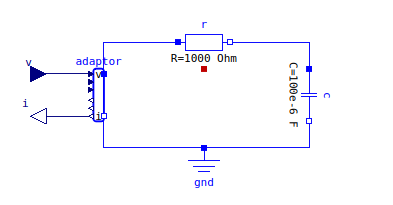
\includegraphics[width=0.5\textwidth]{OmRcModel.png}
\caption{\label{fig:ModelicaModel}Reference RC Series Model.}
\end{figure}
\newline
The parameters used for the model are:
\newline
R = 1000 ohm
\newline
C = 100  uF
\newline
Input of the model is voltage v(t) and output is the current i(t) flowing in the circuit.

\subsection{fmi-interface-cpp}
This library written by Dr. Terraneo can be used to load one or more generic FMI compliant models in a C++ written program. 
Complete source files can be found at (https://github.com/fedetft/fmi-interface-cpp).


\section{Design and Implementation}

\subsection{Equivalent Model}
As a first step a model equivalent to the reference one. Some RC series sample model is already available in Matlab environment (ssc\textunderscore rc\textunderscore circuit\textunderscore sl) so this one will be used as starting point for developing the equivalent model. After some modifications the final model is reported in Figure 2.
\newline
\begin{figure}[h]
\centering
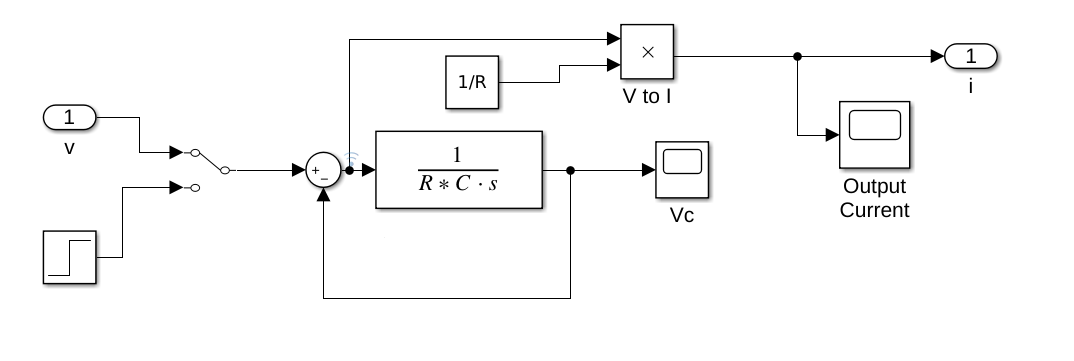
\includegraphics[width=1.0\textwidth]{SimulinkModel.png}
\caption{\label{fig:EquivalentModel}Equivalent RC Series Model.}
\end{figure}

As the reference model, the input is the voltage $v_i(t)$ and the output is the current flowing $i(t)$ in the circuit. 
\newline
Some remarks: the step block before the switch is normally disconnected and has been used for testing purposes only. 
\newline
The voltage drop on the capacitor $v_c(t)$ is computed as follows:
$$v_c(t) = v_i(t)(1 - e^{-t/RC})$$
Which in Laplace domain becomes:
$$V_c(s) = V_i(s)\frac{1}{1 + sRC}$$
In the model this is implemented as:
$$V_c(s) = (V_i(s)-V_c(s))\frac{1}{sRC}$$
After some simple algebraic manipulation:
$$V_c(s) = \frac{V_i(s)}{sRC}\frac{sRC}{1 + sRC}$$
Simplyfing the quantity $sRC$ we get the first expression.
\newline
The summing node computes the quantity $$v_r(t) = v_i(t) - v_c(t)$$
To obtain the current flowing we can apply Ohm law as: $$i(t) = 	\frac{v_r(t)}{R}$$
Substituing all the previously obtained relation we obtain in time domain:
$$i(t) = 	\frac{v_i(t)e^{-t/RC}}{R}$$
In Figure 3 the model ouput is reported. The output is obtained by injecting a Step input signal of 1 V a time t = 1s. As expected at t = 1s the current peaks and is equal to 1 mA since for very high frequency the capacitor can be modeled as a short circuit ($I = V/R$). 
\newline
As t increases the impedence of the capacitor increases and the current exponentially decreases and becomes zero with a time constant $t = RC$  as the capacitor can be assumed to be an open circuit for very low frequency.
\newline
\begin{figure}[ht]
\centering
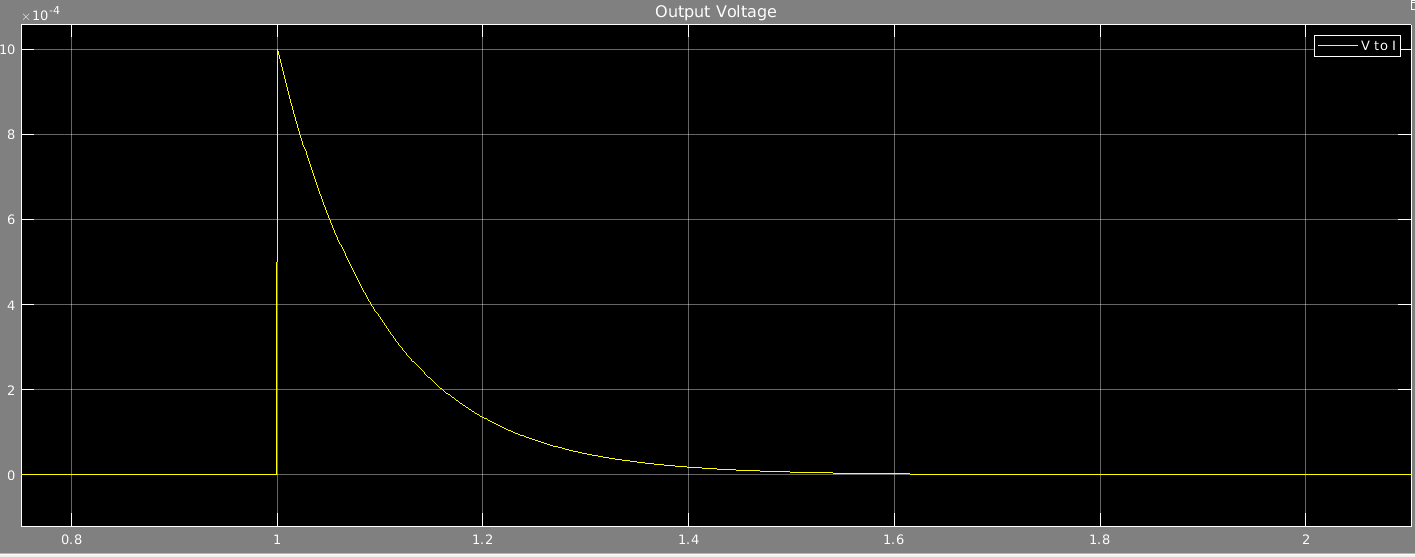
\includegraphics[width=1.0\textwidth]{SimulinkModelOut.png}
\caption{\label{fig:EquivalentModelOutput}Simulink Model Output.}
\end{figure}
\newline
To ensure the two models (Modelica and Simulink) equivalence, a further validation step is performed exploiting Simulink capabilities to import an FMI compliant model. The two model shall be imported in a project then the same voltage signal will be injected and the two output currents will be then compared.
\newline
To import an FMU select Simulink Library browser:
\newline
\begin{figure}[ht]
\centering
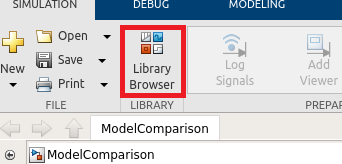
\includegraphics[width=0.5\textwidth]{LibBrowser.png}
\end{figure}
\newline
In the Library browser look for the FMU import block
\newline
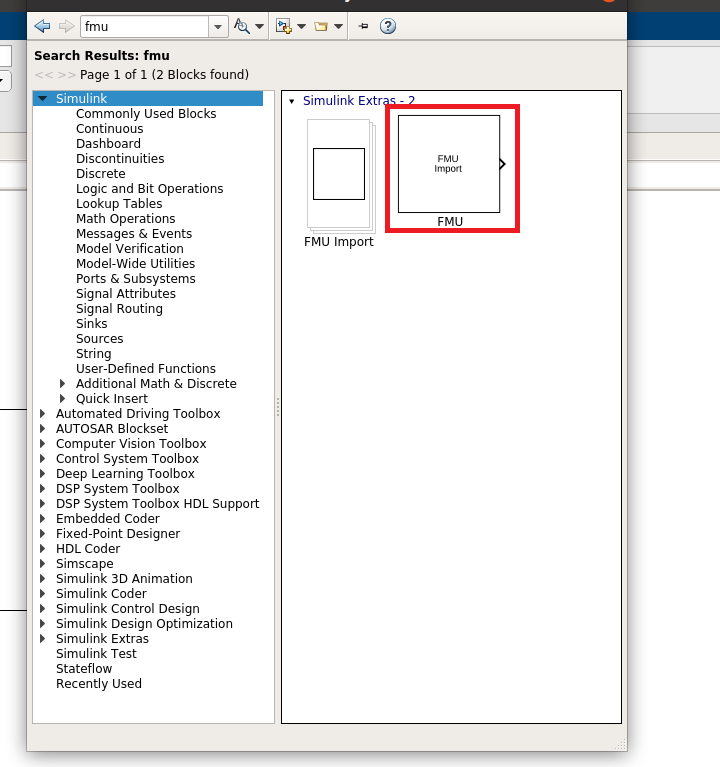
\includegraphics[width=1\textwidth]{FmuImport.png}
\newline
After adding the module into the workspace simply insert the path of .fmu archive that you need to import. 
\newline
NOTE: since OpenModelica does not output a .fmu, first add into a comppresed archive to generated Model(.xml and .so are needed) then change to extension to .fmu.
\newline
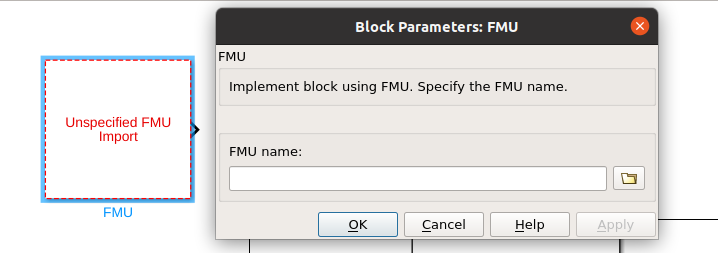
\includegraphics[width=1\textwidth]{FmuImport2.png}
\newline
\newline
The two models are then imported in the workspace as shown in figure 4
\newline
\begin{figure}[ht]
\centering
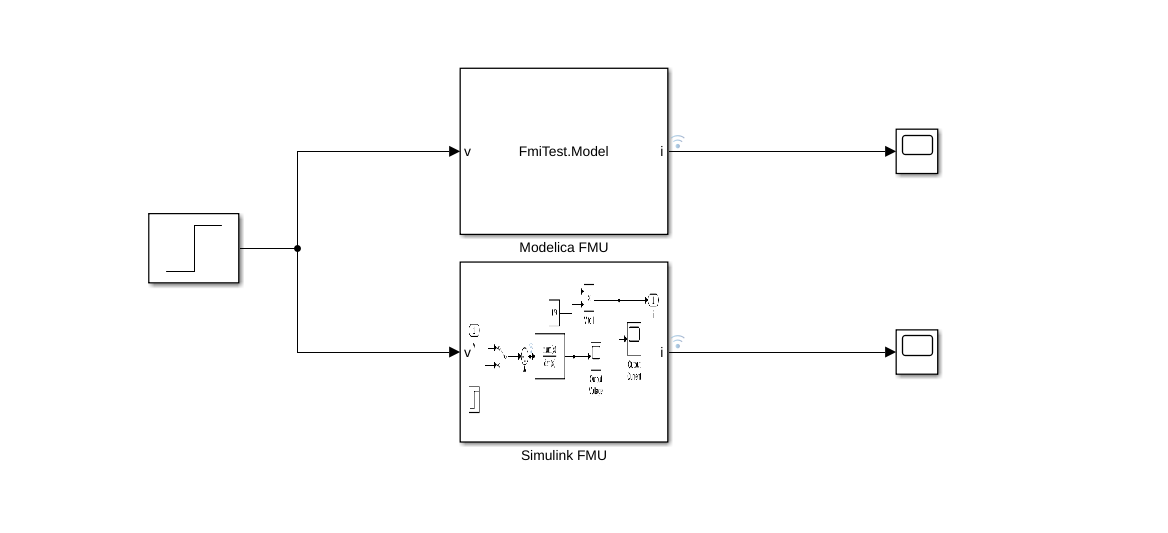
\includegraphics[width=1.0\textwidth]{ModelComparison.png}
\caption{\label{fig:ModelComparison}Model Comparison.}
\end{figure}

By injecting the same voltage signal no notable difference can be observed on the two outputs as reported in figure 4.
\newline
\begin{figure}[ht]
\centering
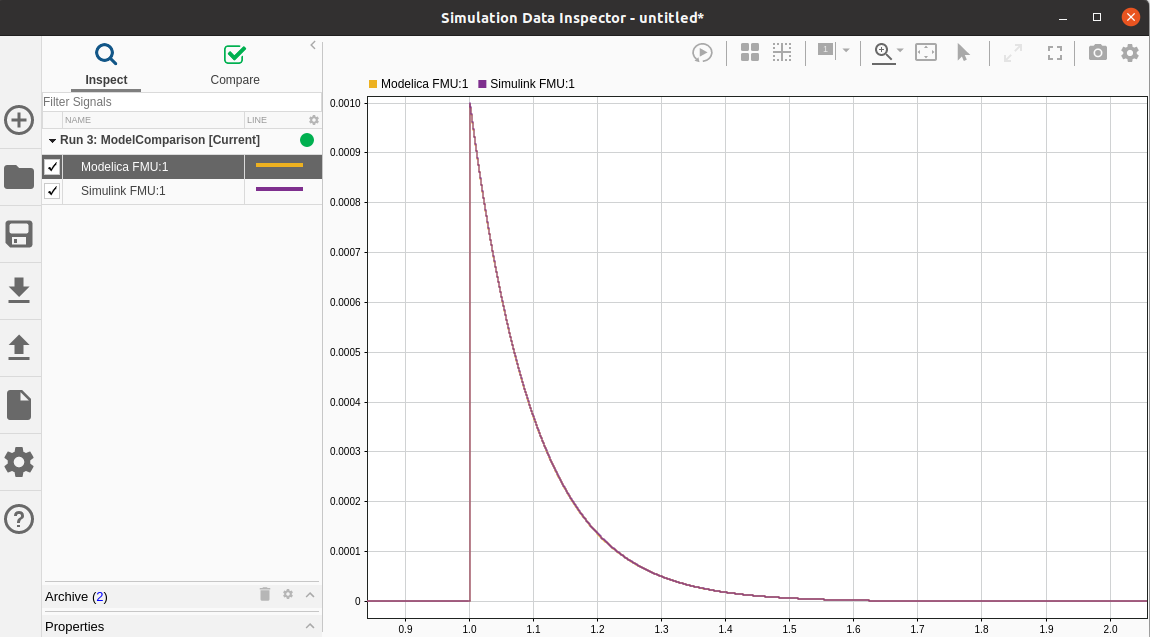
\includegraphics[width=1.0\textwidth]{ModelComparisonOutput.png}
\caption{\label{fig:ModelComparison}Model Comparison Output.}
\end{figure}
\newpage
\subsection{FMU Generation using Simulink}
To generate a standalone FMU from the developed model the following steps needs to be performed. 
First the solver type must be set to "Fixed Step". 
\begin{center}
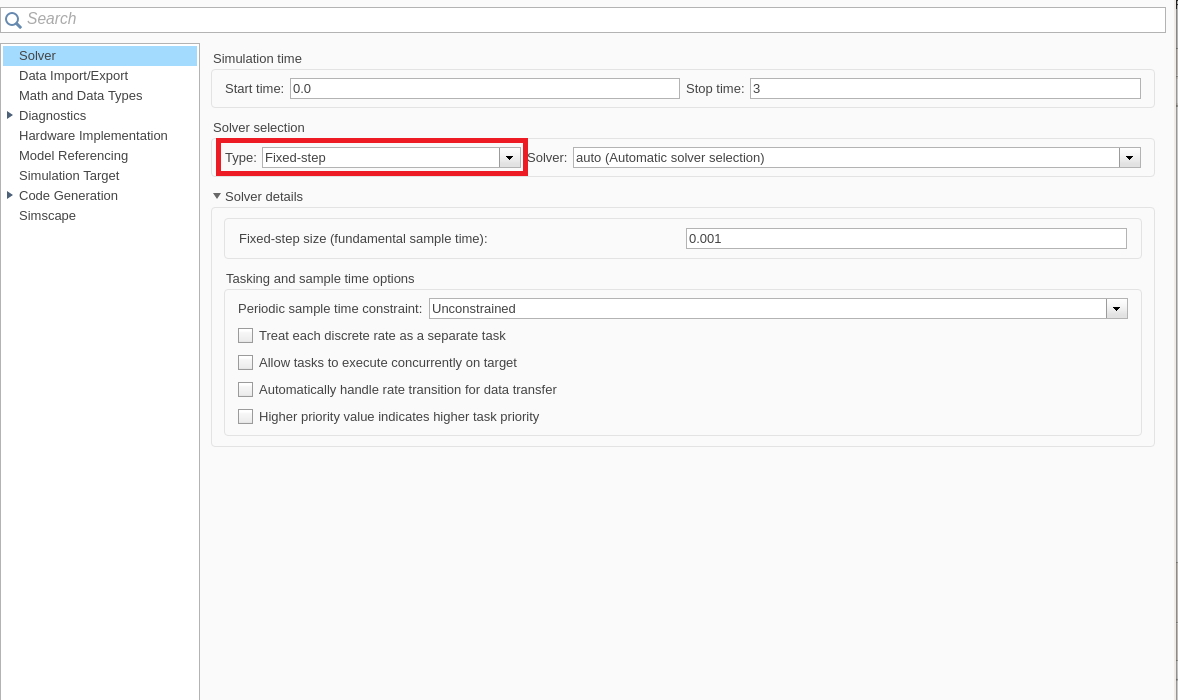
\includegraphics[width=0.9\textwidth]{Solver.png}
\end{center}
NOTE: When the model is run as FMU in a C++ program, is not possible to use a step size which is lower then the one selected as Step size in the Simulink Model, so care must be taken regarding the selection of this parameter.
\newline
The next step is to generate a FMU standalone using Simulink exporting tool from Simulation $\rightarrow$ Save $\rightarrow$  Standalone FMU:
\begin{figure}[ht]
\centering
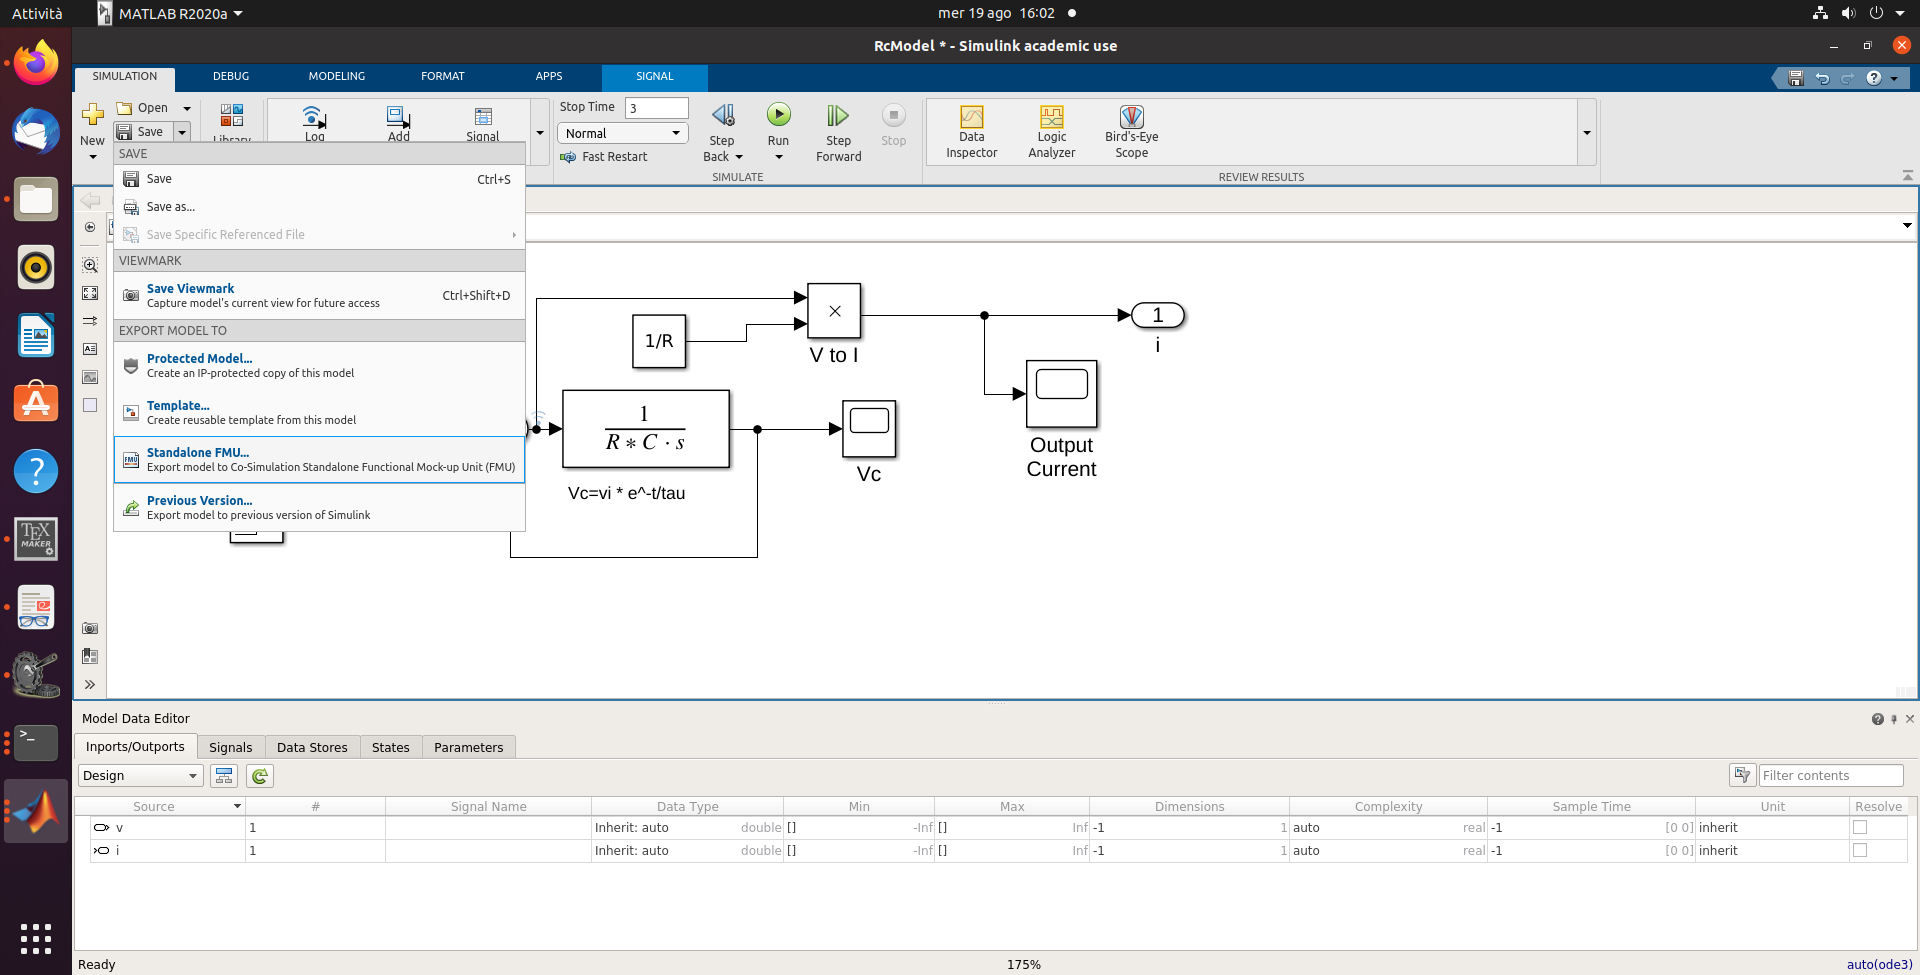
\includegraphics[width=1.0\textwidth]{FmuExport1.png}
\end{figure}
\newline
The following window is shown. Choose the export path then select Create.
\newline
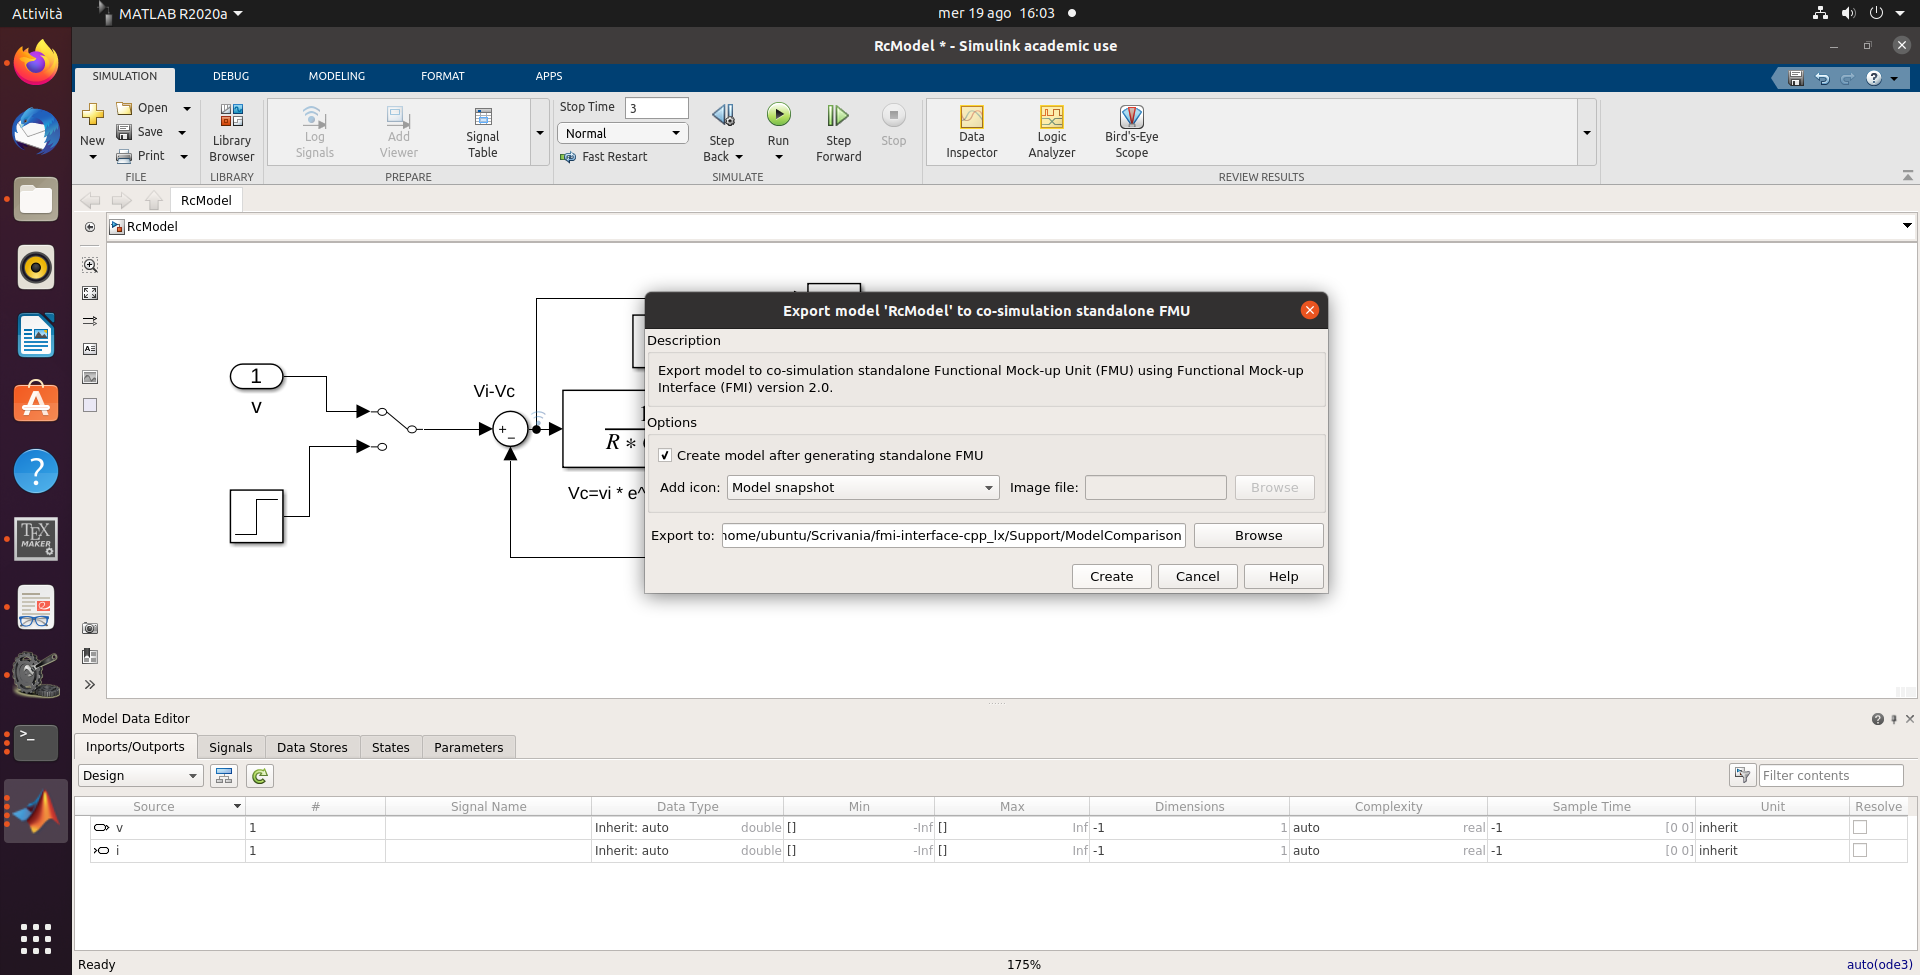
\includegraphics[width=1.0\textwidth]{FmuExport2.png}
\newline
If no error is detected in the generation phase, the ouput of this export operation shall be a .fmu compressed archive that contains the .xml descriptor and .so library of the model ( optionally if selected in the export phase a .png report a model graphical snapshot )
\newline
\newline
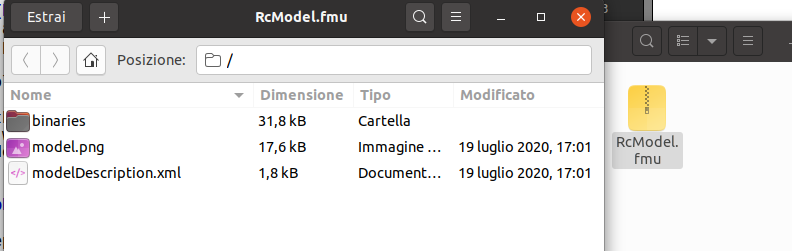
\includegraphics[width=1.0\textwidth]{OuputModel.png}
\newline
In this case we get a RcModel.fmu and RcModel.so in the binaries folder ( the library is generated with the same name as .fmu).
\newline
The last step is to decompress the .fmu archive.

\subsection{Model load using fmi-interface-cpp}
To load this new obtained model and compare the simulation results with the Modelica model, the start point will be the program fmitest.cpp ( available in fmi-interface-cpp project repository ). This program loads the sample Modelica RC model and run a simulation of duration 1 s with a step of 10 ms and at t = 100 ms injects a step voltage of 1 V. At every simulation step $n$ the input $v_i(n)$ and the output $i(n)$ is printed on the console.
\newline
First a new object of class FmiInterface initialized with RcModel is declared.
\begin{verbatim}
    // Load the Simulink Rc Model
    FmiInterface fmiSimulink("RcModel","../",LogLevel::Normal);
\end{verbatim}

Then the code used for the Modelica model is simply replicated for the object fmiSimulink (printVariables, getting v and i index and startSimulation )

\begin{verbatim}
    fmiSimulink.printVariables();
    auto vSimulinkIndex=fmiSimulink.variableIndex("v");
    auto iSimulinkIndex=fmiSimulink.variableIndex("i"); 
    fmiSimulink.startSimulation();
\end{verbatim}

After this initial startup the Input is set using the same variable as Modelica model and the step is performed using the same time variables.

\begin{verbatim}
    fmiSimulink.setScalarDouble(vSimulinkIndex,v);
    fmi.setScalarDouble(vIndex,v);
    
    fmiSimulink.doStep(time,step);
    fmi.doStep(time,step);
\end{verbatim}
An additional modification to allow simple csv log of the system variable for post elaboration and verification has been added to fmitest.cpp.
\section{Experimental Results}
Below the a Matlab generated plot obtained from .csv is reported:
\begin{figure}[ht]
\centering
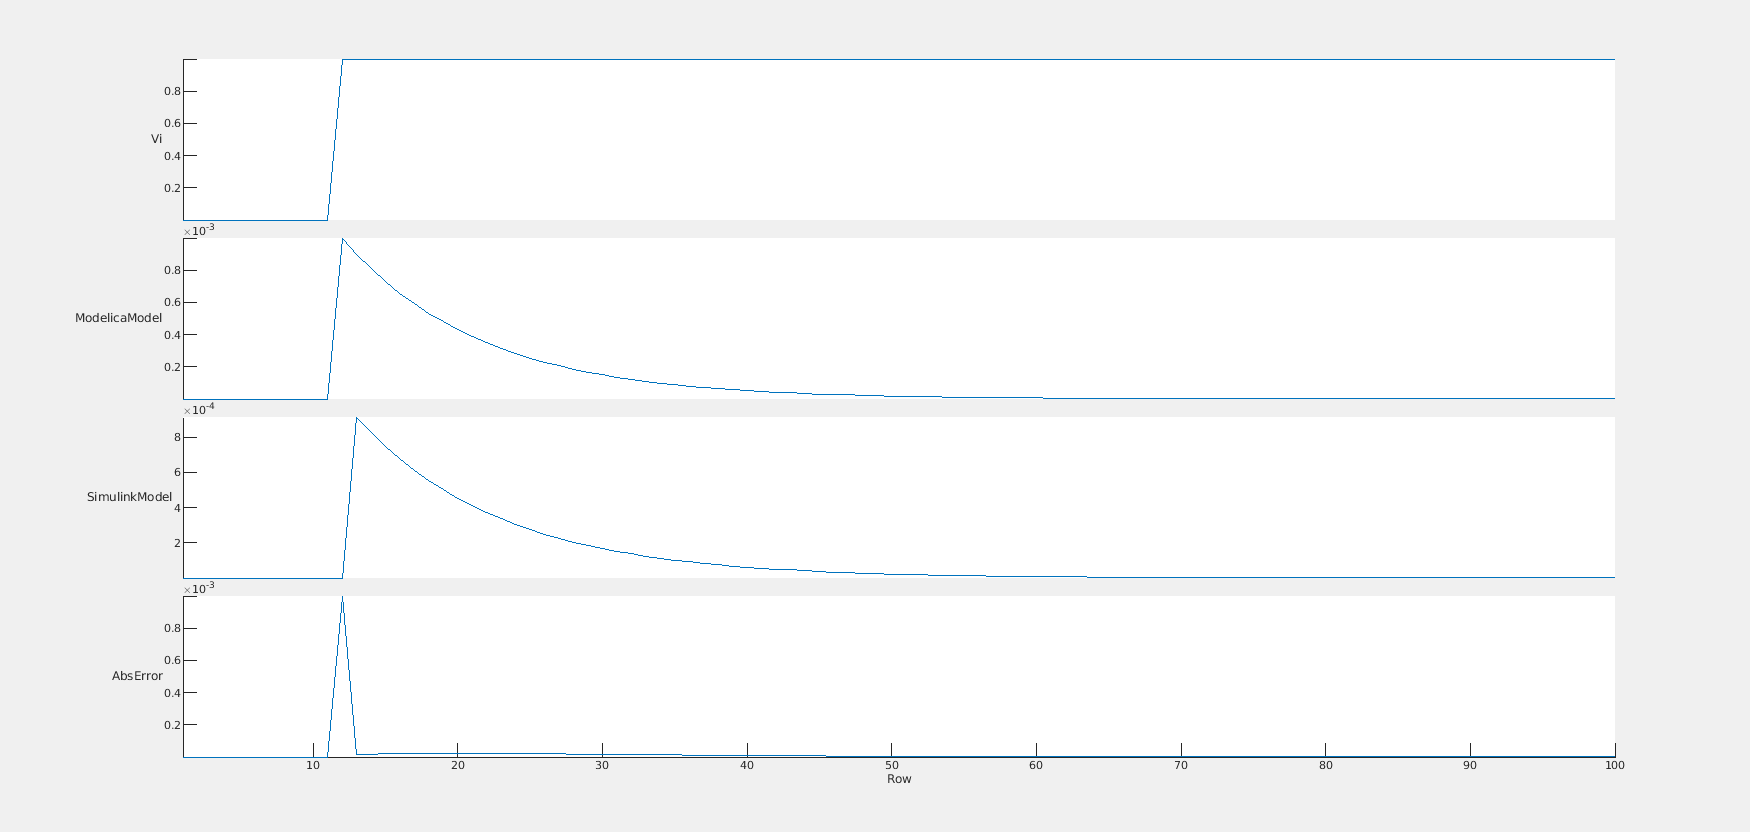
\includegraphics[width=1.0\textwidth]{CsvComparison1.png}
\caption{\label{fig:ModelComparison}Experimental results.}
\end{figure}
The first plot is the input $v_i(n)$ , the second and the third plots reports $i(n)$ computed with the reference Modelica Model and the equivalent Simulink Model. The last plot reports the absolute error between the computed $i(n)$ of the two models.
\newline
As can be seen from the asolute error plot, the two model behaviour does mostly agree excepts for the simulation step when voltage step is injected. This behaviour is probably due to some difference in the generated Simulink FMU.
\newline 
Apparently the algebraic part of the system is better managed by the Modelica generated model since when the input voltage step is injected, the current in the circuit should immediatly change, this correctly happens in the reference model, while in the Simulink model it is required that at least a simulation step is completed. 
\newline
From the plots, we can see that at n=12, the step voltage is injected and the reference model reacts immediatly. The Simulink model reacts at n=13 but the delay is not a simulation step (10 ms), but the chosen fixed step size of the model (1 ms), this explains why the Simulink plotted output does not reach the 1 mA value as expected but nearly 0.9 mA 

\begin{figure}[ht]
\centering
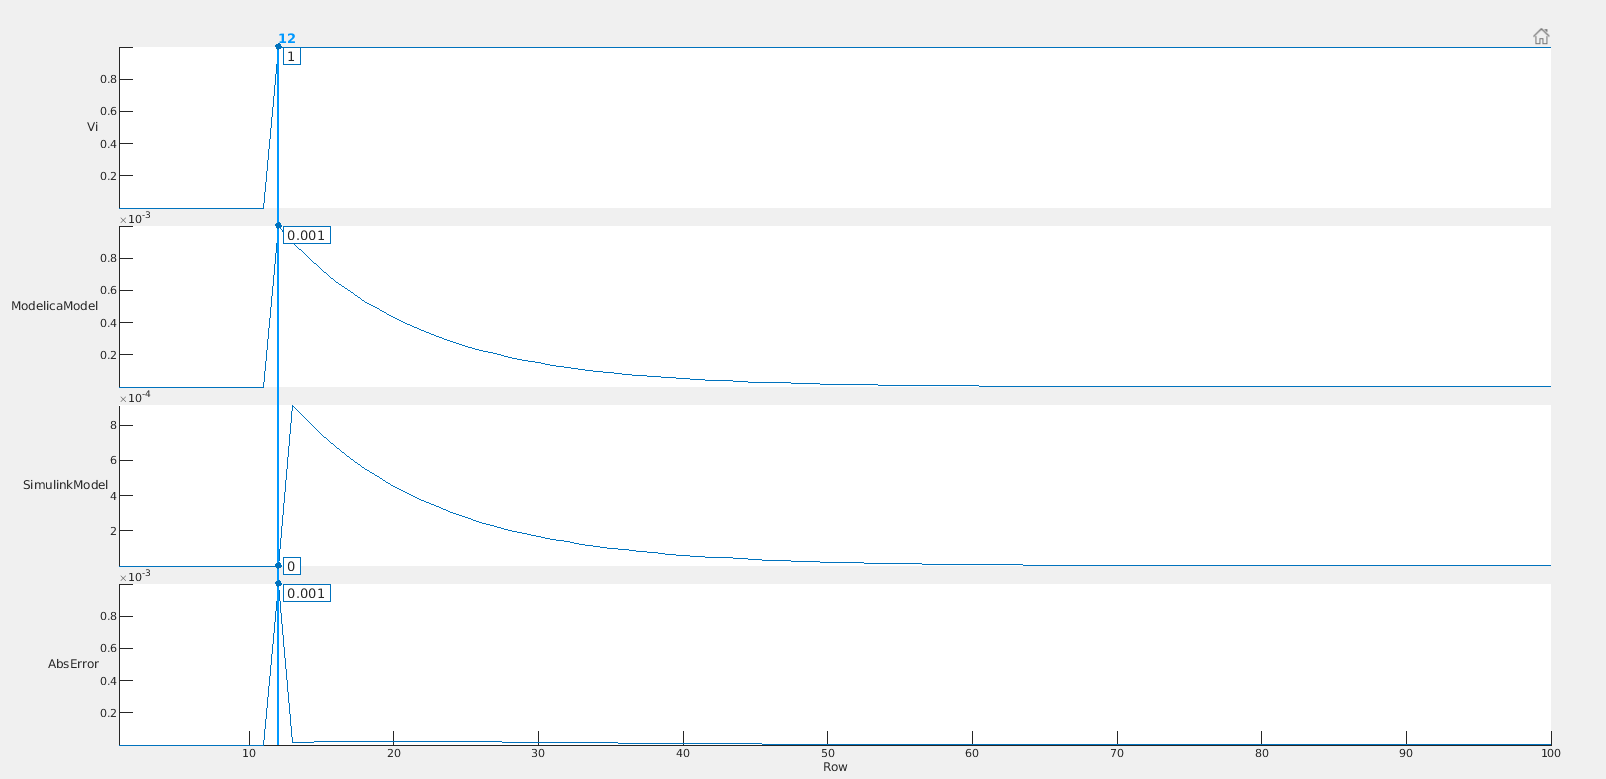
\includegraphics[width=1.0\textwidth]{CsvComparison2.png}
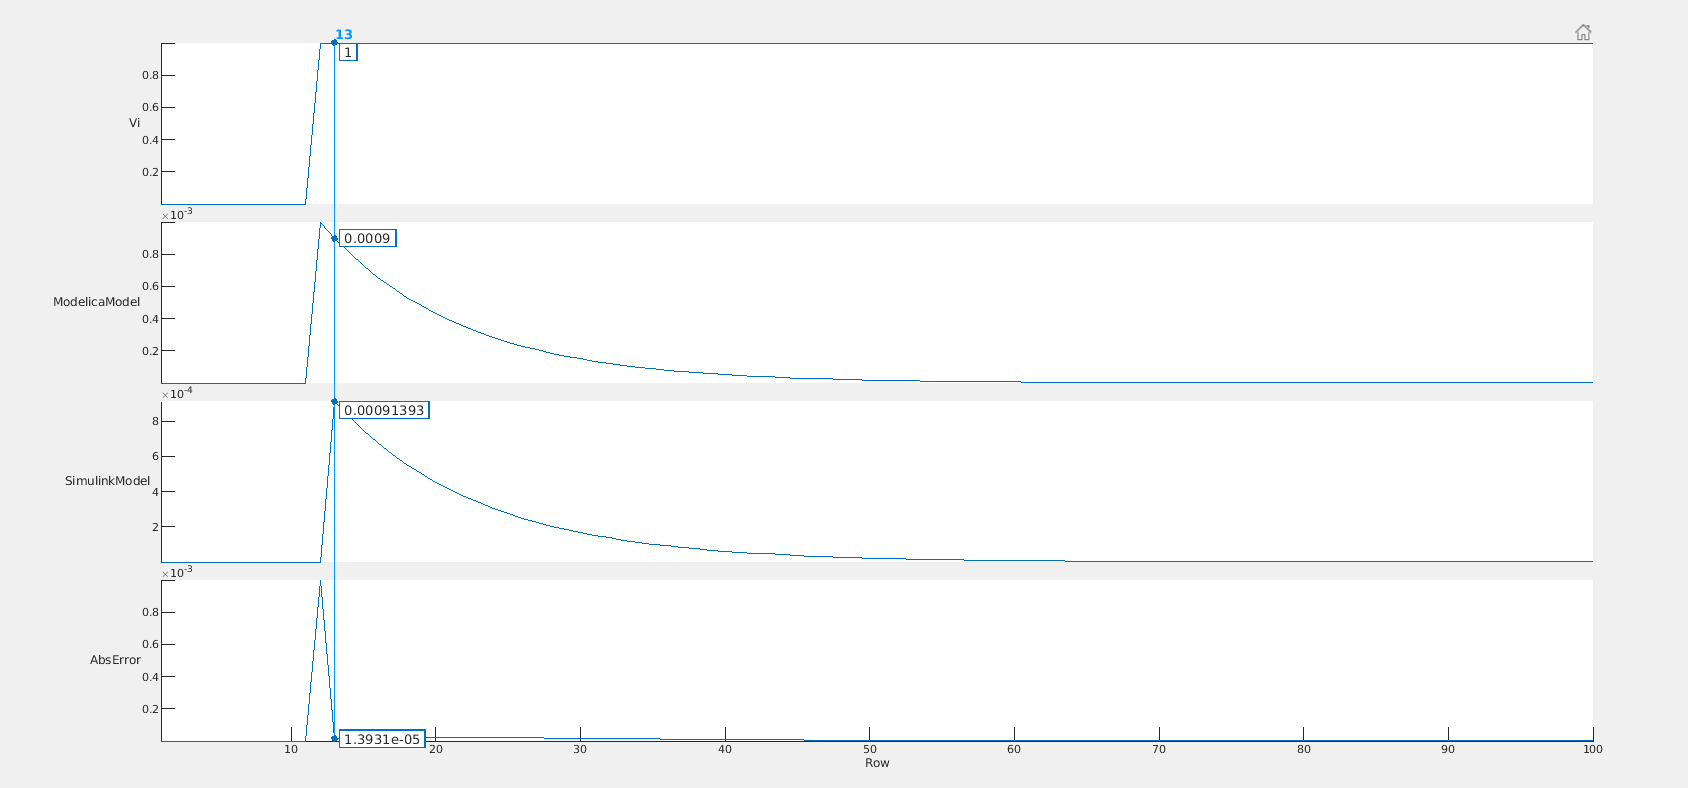
\includegraphics[width=1.0\textwidth]{CsvComparison3.png}
\end{figure}
This conclusion can verified by changing the simulation step in fmitest.cpp from 10 ms to 1 ms.
\begin{figure}[ht]
\centering
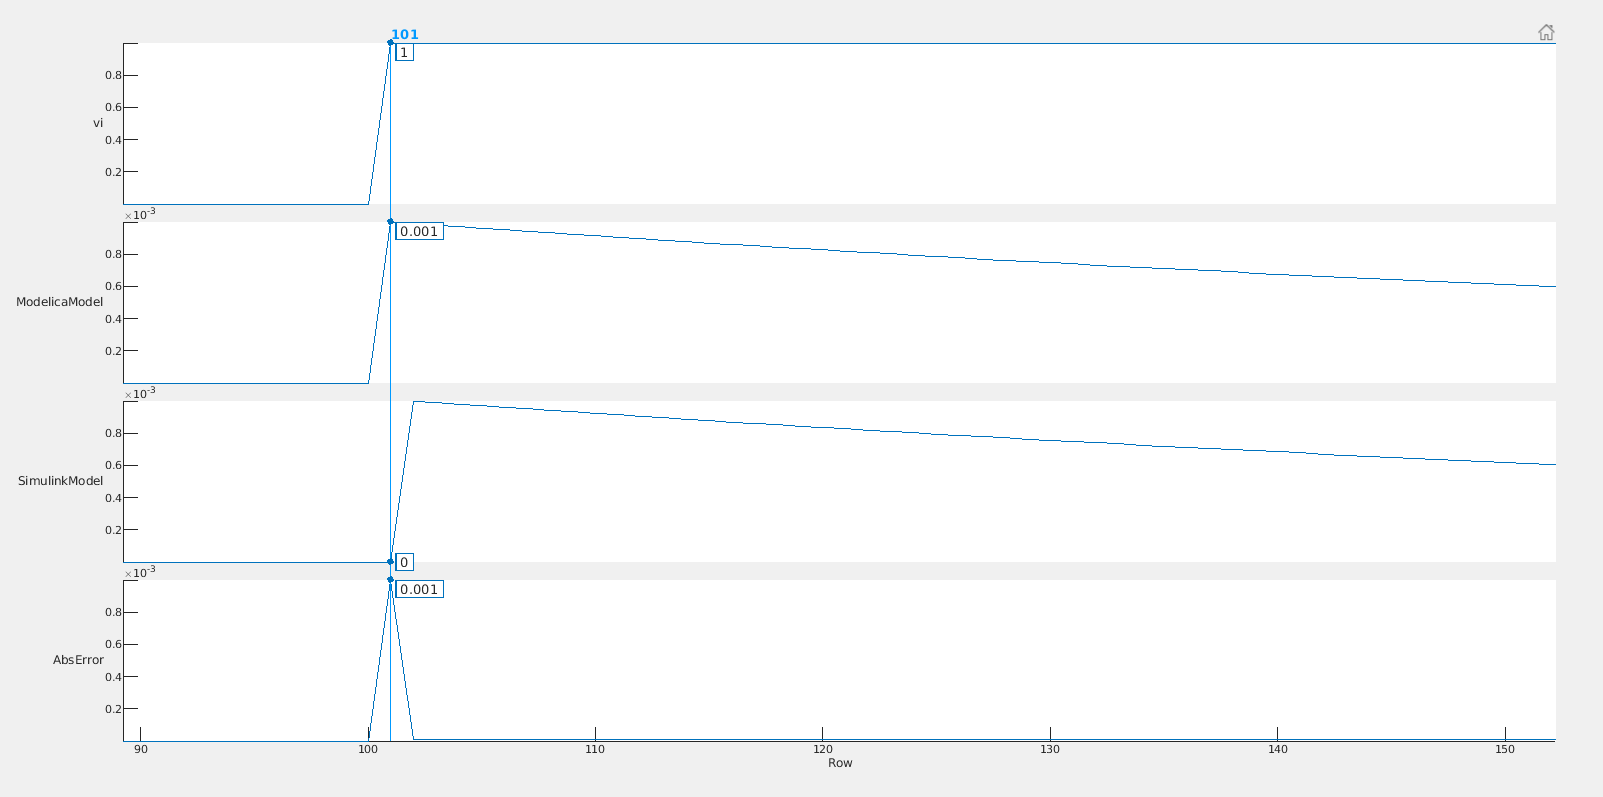
\includegraphics[width=1.0\textwidth]{CsvComparison4.png}
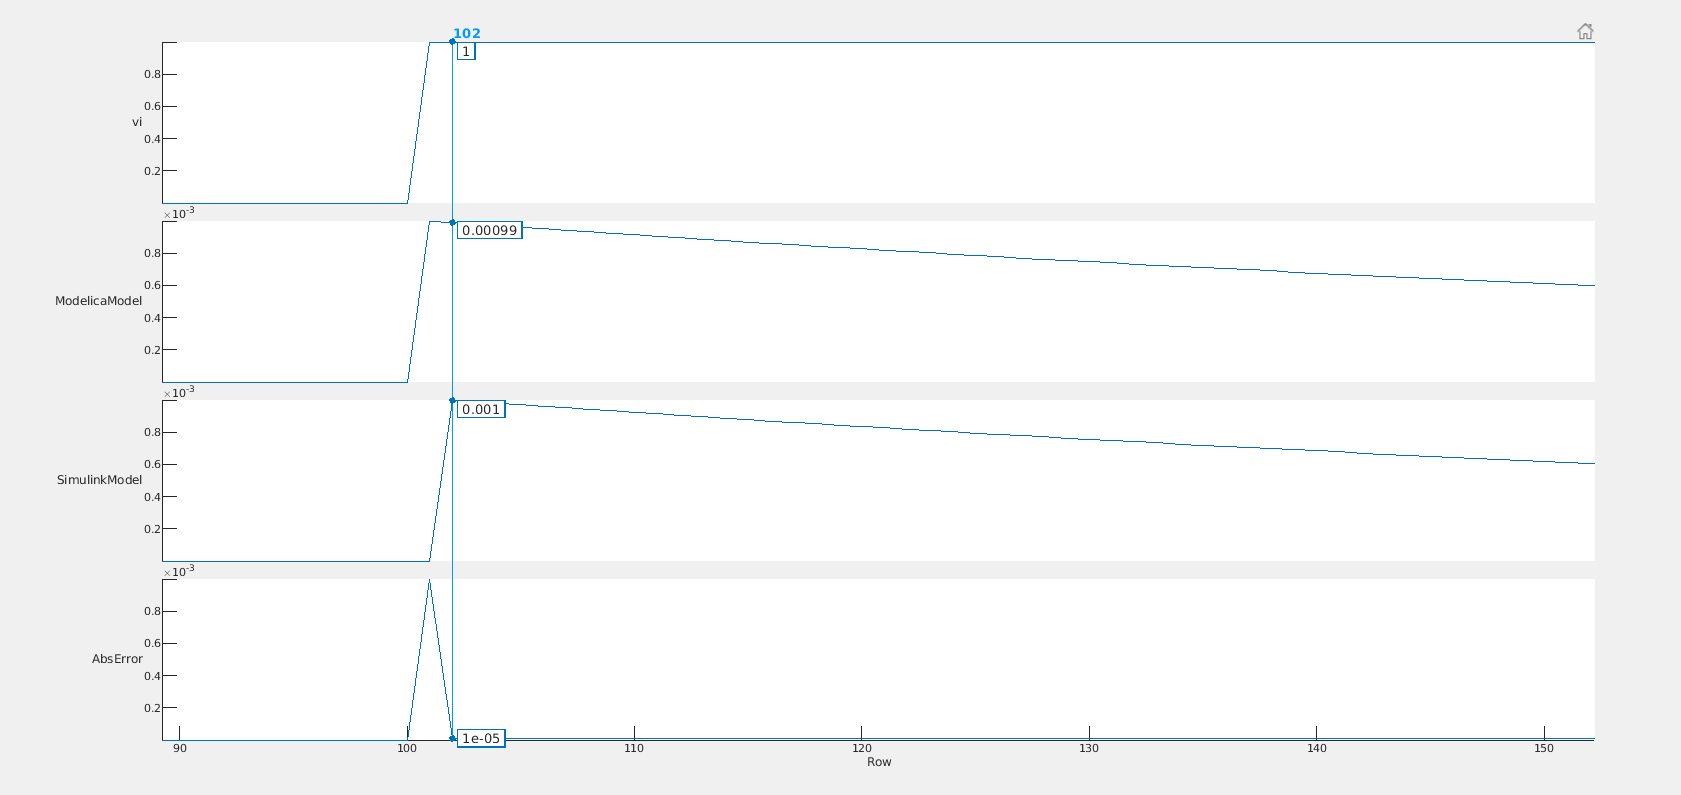
\includegraphics[width=1.0\textwidth]{CsvComparison5.png}
\end{figure}
Using this simulation step, we can se that at n = 101 the voltage step is injected, an the behaviour is the same as the previous case. At n = 102 the Simulink model reacts to the input this time reaching the current of 1 mA.
After this step, the Simulink model is always beyond one simulation step in respect to the reference model.
\section{Conclusions}

The generation of a standalone FMU from Simulink has been carried out. The package has been then succesfully imported in a C++ program using the library fmi-interface-cpp. Some discrepancy in the generated model in respect to the reference model has been noted, but this is most probably due to Simulink generated code ( needs at least a simulation step before update the input state ). 
\newline 
This difference shouldn't be a problem if all the FMU models used are Simulink generated, but even in a mixed-tool model environment the differences could be not noticable ( dependes on the modeled systems and simulation objectives ).
\newline
More complex and advanced models comparations are needed to evaluate and highlights further possible differences between the two tools code generation alghoritms.
\end{document}